\documentclass{article}
\usepackage{graphicx}
\usepackage{minted}
\usepackage{parskip}
\usepackage[colorlinks,
            urlcolor=blue]{hyperref}
%\usepackage[margin=1in]{geometry}
\usepackage{amsmath}
\usepackage{amssymb}
\usepackage{fancyvrb}
\usepackage{booktabs}
\usepackage{url}
\usepackage{hyperref}
\usepackage{multirow}
\usepackage{pbox}
\usepackage[margin=1in]{geometry}

\author{Ashwin Srinath}
\title{An OpenCL-based tridiagonal solver for evaluation
    of compact finite differences on parallel architectures}
\begin{document}
% \renewcommand{\bibname}{References}

\section{Introduction}

    The motivation for this work comes from the need to evaluate
    \emph{compact finite differences} arising in large simulations of combustion.
    Compact finite different schemes result in
    high-order of accuracy for relatively small stencils.
    Numerical methods with small stencil widths are especially benefitial
    in managing communication costs in large-scale cluster computing.
    This work is concerned with implementing algorithms for evaluating
    compact finite differences to make full use of available parallel architecture.
    The target architecture studied is the NVIDIA Tesla K20 GPU.
    The algorithm design for this architecture is presented,
    along with the associated issues.
    Results are presented for domains sized up to $2048^3$ grid points,
    using up to 64 GPUs.

\section{Related work}

    [FastTridiagonal] discuss the GPU implementation of three algorithms
    and their hybrid variants: Cyclic Reduction, Parallel Cyclic Reduction
    and Recursive Doubling.
    Their approach utilizes the GPUs \emph{shared memory},
    and addresses the concerns of bank conflicts arising in these algorithms.
    A global memory implementation of their solvers
    runs about three times slower, but is able to accomodate larger systems.
    The speedups they report are 12x over a 2.5 GHz quad-core CPU.

    [ScalableTridiagonal] and [Autotuned] both propose hybrid
    Parallel Cyclic Reduction and thread-level parallel Thomas algorithm (p-Thomas), and
    methods to determine the switching point for the algorithms.
    The speedups reported are 8.3x and 11x over a 3.33 GHz Intel i7 quad-core
    processor and a 3.4 GHz Intel i5 dual-core respectively.

    In [ScalableNumericallyStable],
    the authors implement a heterogenous (GPU+MPI) solver using the
    SPIKE algorithm for GPUs with a diagonal pivoting strategy for stability.
    More recently, [ChunkedCyclic] propose a \emph{chunked} cyclic reduction
    strategy for GPUss
    In [GPUApplicationForHigherOrderCFD], the inverse of the coefficient matrix
    is used to solve tridiagonal systems resulting from high-order compact
    finite difference schemes. The work here is for a single GPU.
    [An efficient GPU implementation of cyclic reduction solver] demonstrate
    a method to improve memory accesses for Cyclic Reduction
    using a reordering strategy, and apply it to compressible viscous flow
    simulations.

    --- Mention the speedups

    In this work, we propose a variant of Cyclic Reduction for solving
    tridiagonal systems arising in compact finite differences
    in a cluster environment (several GPU nodes).
    We introduce a strategy to
    reduce global memory accesses and decrease memory requirements by
    pre-computing coefficients appearing in Cyclic Reduction.


\section{Numerical method}

    We consider the following fourth-order
    compact finite difference scheme for evaluating the first derivative,
    with a 3-point stencil:

    \begin{equation}
        \alpha(f^{\prime}_{i-1} + f^{\prime}_{i+1}) + f^{\prime}_i
        =
        a\frac{f_{i+1} - f_{i-1}}{dx}
    \end{equation}

    For the particular scheme used, $\alpha = 1/4$,
    and $ a = 3/4 $.
    It is easily noted that this leads to a tridiagonal system of equations,
    along with a 3-point stencil to evaluate the RHS.
    Further, the left boundary can be treated using the following implicit equation:

    \begin{equation}
        f^{\prime}_1 + 2f^{\prime}_2 = \frac{-5f_1 + 4f_2 + f_3}{dx}
    \end{equation}

    The right boundary ($f^{\prime}_{n-1}$) is treated by utilizing
    the negative complex-conjugate of the Fourier image of the stencil
    at $f^{\prime}_1$:

    \begin{equation}
        f^{\prime}_{n-1} + 2f^{\prime}_{n-2}
        =
        \frac{5f_{n-1} - 4f_{n-2} - f_{n-3}}{dx}
    \end{equation}

    The tridiagonal system that needs to be solved for the derivatives,
    then has an LHS of the form:

    \[ %\arraycolsep=4pt
     \begin{bmatrix}
         1&2\\
         1/4&1&1/4\\
         &1/4&1&1/4\\
         &&1/4&1&1/4\\
         &&&1/4&1&1/4\\
         &&&&&\ddots\\
         &&&&&&\ddots\\
         &&&&&&&\ddots\\
         &&&&&&&2&1
      \end{bmatrix}
    \]

    And an RHS of the form:

    \[
     \begin{bmatrix}
         -5f_1 + 4f_2 + f_3\\
         f_{3} - f_{1}\\
         f_{4} - f_{2}\\
         \vdots\\
         \vdots\\
         \vdots\\
         \vdots\\
         f_{n} - f_{n-2}\\
         5f_{n} - 4f_{n-1} - f_{3}
      \end{bmatrix}
    \]

    A solution strategy is therefore concerned with the following:

    \begin{enumerate}
        \item{The evaluation of the right hand side.}
        \item{The solution of the resulting matrix system.}
    \end{enumerate}

\section{Reference approach}
    The current approach, developed for the CFDNS[ref] Compressible Navier-Stokes,
    and adapted to the Roadrunner[ref] architecture,
    is a parallel solver based on the standard LU algorithm,
    but specialized for the solution of a constant matrix.
    The problem is distributed among several ``processes'' and each
    process uses a single CPU core to perform computations.

    Assuming the coefficients of the LU algorithm are precomputed,
    the following steps are required to solve the tridiagonal system
    (only steps for the left-right sweep are listed, the right-left sweep
    consists of similar steps):

    \begin{enumerate}
    \item Precompute the arrays of coefficients of the LU algorithm---
    this is done once, in the beginning of the simulation process, and its cost
    can be neglected.
    \item Evaluate the RHS of the system.
    \item Compute $\hat{\phi_i}$ and $\hat{\psi_i}$ for each grid point $i$,
    with $\hat{\phi_i}$ and $\hat{\psi_i}$ both functions of the precomputed
    coefficient arrays and the right hand side.
    \item Every process posts the rightmost values of its $\hat{\phi_i}$ and $\hat{\psi_i}$,
        $\widetilde{\phi_k}$ and $\widetilde{\psi_k}$.
    \item Using the array of $\widetilde{\phi_k}$ and $\widetilde{\psi_k}$,
        each process computes $\widetilde{x_k}$, and uses it to compute
        $x_i,k = \phi_i + \psi_i\widetilde{x_k}$.
    \end{enumerate}

    The Message Passing Interface (MPI) is used for handling communication
    between processes.

\section{GPU architecture and OpenCL programming platform}

    \begin{figure}[h]
    \begin{center}
    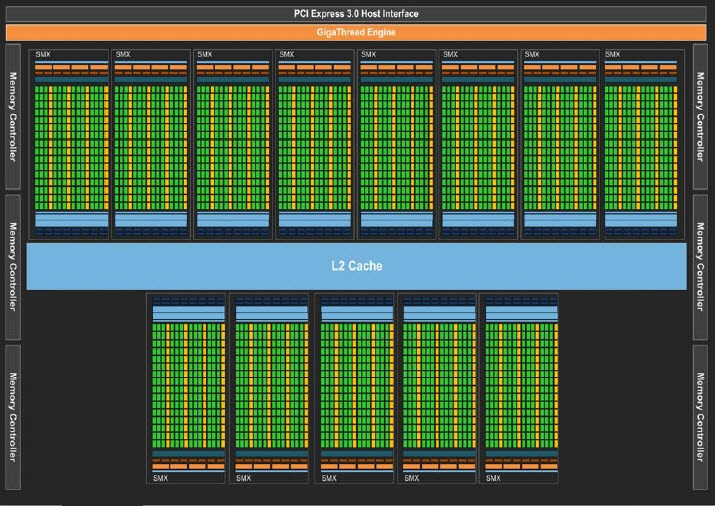
\includegraphics[height=200pt]{img/tesla-block-diagram.jpg}
    \end{center}
    \caption{Distribution of a 2-D domain among processes}
    \label{fig:da-domain}
    \end{figure}

    GPUs afford massive parallelism by virtue of several (thousand)
    lightweight compute threads, referred to as \emph{work items}.
    The work items on a GPU are scheduled as \emph{blocks},
    which can be 1-D, 2-D, or 3-D.
    Each block is assigned to a \emph{streaming multiprocessor} (SM)
    on the GPU---the Tesla K20 GPU has 13 streaming multiprocessor---and
    all threads in a block are executed simultaneously by the SM.
    All SMs (and therefore all threads) have access to the GPU's ``global'' memory.
    Access to global memory is efficient when concurrent threads
    access neighbouring memory locations
    (known as \emph{coalesced memory access}).
    All threads in an SM also have access to a common fast, on-chip, \emph{shared memory}.
    Access to shared memory, in general, is much faster than access to global memory,
    but the amount of shared memory per SM is limited, typically a few dozen KB.
    Certain memory access patterns by concurrent threads to shared memory may result in
    serialization of the memory accesses, known as bank conflicts. These are detailed [here].

\section{Parallelization strategies}


    % left, lower, right, upper
    \begin{figure}[h]
    \begin{center}
    \includegraphics[trim={{100pt} {150pt} {100pt} {150pt}}, clip, height=250pt]{img/domain.eps}
    \end{center}
    \caption{Problem domain}
    \label{fig:domain}
    \end{figure}

    \begin{figure}[ht]
    \begin{minipage}[b]{0.45\linewidth}
    \centering
    \includegraphics[trim={{50pt} {150pt} {50pt} {150pt}}, clip, height=200pt]{img/one-block.eps}
    \caption{Single block assigned to a process}
    \label{fig:block}
    \end{minipage}

    \hspace{0.5cm}
    \begin{minipage}[b]{0.45\linewidth}
    \centering
    \includegraphics[trim={{50pt} {150pt} {50pt} {150pt}}, clip, height=200pt]{img/one-thread.eps}
    \caption{Single grid line within a block}
    \label{fig:grid-line}
    \end{minipage}
    \end{figure}

    The compact finite differences need to be evaluated
    at each grid point in the problem domain,
    shown in \ref{fig:domain}.
    Each grid point is represented as a cell in this representation.
    The domain has been shown as partitioned into blocks \ref{fig:one-block}.
    The blocks are three dimensional to facilitate
    the computation of derivatives in all three coordinate directions
    without incurring excessive communication costs.

    While evaluating the derivative in the x-direction (say),
    each block is assigned to a \emph{compute unit}, or a \emph{process}
    which may be a single core, a multi-core processor, or a GPU.
    Each block may be thought of as a collection of ``lines'' of grid points
    \ref{fig:one-line}---referred to as \emph{grid lines}---in the x-direction,
    and the entire domain may be thought of as a collection of such blocks.

    \subsection{Evaluation of the RHS}

        The RHS is evaluated by a 3 point stencil computation of
        the following form:

        \begin{equation*}
            r_i = \frac{3}{4dx} (f_{i+1} - f_{i-1})
        \end{equation*}

        This pointwise update can be performed easily in parallel
        for the internal points (points not close to the boundary of the process).
        Near the boundaries, the process will require information from its
        neighbours.

        Thus, each process will require information from its
        neighbouring processes every time the derivative needs to be evaluated.

        \begin{figure}[h]
        \begin{center}
        \includegraphics[trim={{100pt} {250pt} {100pt} {200pt}}, clip, height=200pt]{img/da-domain.eps}
        \end{center}
        \caption{Distribution of a 2-D domain among processes}
        \label{fig:da-domain}
        \end{figure}

        \begin{figure}[h]
        \begin{center}
        \includegraphics[trim={{100pt} {250pt} {100pt} {200pt}}, clip, height=200pt]{img/da-local-portion.eps}
        \end{center}
        \caption{Elements required by a process to evaluate RHS}
        \label{fig:da-local-portion}
        \end{figure}

        Thus, the RHS is evaluated in two steps:

        \begin{enumerate}
            \item Exchange boundary information with neighbouring processes
            \item Evaluate the RHS at each grid point (in parallel)
        \end{enumerate}

        The GPU is specialized for performing such a large number of independent
        computations as required in step 2.
        The RHS at each grid point is computing by a single work item
        (GPU thread).
        Therefore the number of work items scheduled is
        equal to the number of points in the local domain.

        Another popular strategy is to take advantage of
        shared memory, by launching 2-dimensional blocks of work-items,
        loading each into shared memory, and streaming the third dimension
        in registers.
        This approach is discussed in [ref], and is much more effective
        for larger stencils---as each thread in a block will access the same
        value several times, it is effective to use shared memory as explicitly
        controlled cache.

    \subsection{Solving the tridiagonal system}

        In the reference approach, a significantly larger portion of time is spent in solving
        the tridiagonal system in parallel.
        Because the problem does not exhibit the same degree of parallelism as
        the pointwise stencil update,
        the algorithms are necessarily more involved.

        \begin{figure}[h]
        \begin{center}
        \includegraphics[trim={{100pt} {150pt} {100pt} {150pt}}, clip, height=250pt]{img/block-dimensions.eps}
        \end{center}
        \caption{Domain}
        \label{fig:block-dimensions}
        \end{figure}

        In the reference approach, the domain is decomposed into several blocks,
        and each block is assigned to a CPU core.
        Each core operates on a block with dimensions as shown
        in the figure \ref{fig:block-dimensions}.
        The computational pattern followed by each core for the steps listed in Section[SEC]
        is a triple nested loop over the grid points in the block,
        followed by a communication of the ``faces'' of the block with the other
        cores:

        \begin{listing}
        \begin{minted}{fortran}
           do j=1,n2
              do i=1,n1
                 x(1,i,j) = bet(1)*x(1,i,j)
                 do k = 2, n3
                    x(k,i,j) = (x(k,i,j) - a(k)*x(k-1,i,j))*bet(k)
                 end do
                 p_loc(i,j) = x(n3,i,j)
              end do
           end do

           call MPI_Allgather(p_loc,n1*n2,double_real,p,n1*n2, &
              double_real,comm,error)

        \end{minted}
        \caption{Computational pattern in reference approach}
        \end{listing}

        Conceptually, the innermost loop solves the tridiagonal system
        for a single ``line'' of grid points.

        In a multi-threaded environment,
        rather than having a single thread perform the local part
        of the computations for each line,
        it is beneficial to have several threads ``sweep'' through the domain,
        each performing the computations for a different tridiagonal system.
        This is shown in Figure \ref{fig:block-multi-threaded} for a 4-core processor.
        In each iteration of the inner-most loop,
        4 lines of grid points are solved.

        \begin{figure}[h]
        \begin{center}
        \includegraphics[trim={{50pt} {250pt} {50pt} {150pt}}, clip, height=300pt]{img/block-multi-threaded.eps}
        \end{center}
        \caption{Domain}
        \label{fig:block-multi-threaded}
        \end{figure}

        Algorithms like LU and the Thomas Algorithm are inherently sequential.
        While thread level parallelism can be used to solve several systems at once,
        the number of steps to solve each system remains large.

        Algorithms like Cyclic Reduction and Parallel Cyclic Reduction use
        several parallel processors to solve a tridiagonal system.
        Cyclic reduction

\section{Description of the algorithm}

    First, we discuss the cluster level parallelism.

    Given N equations in N variables of the form:

    \begin{align}
    & A =
     \begin{bmatrix}
         b_1 & c_1 \\
         a_2 & b_2 & c_2 \\
             & a_3 & b_3 & c_3 \\
             &     & a_4 & b_4 & c_4 \\
             &     &     &     &  \ddots & c_{N-1}\\
             &     &     &     &     a_N  & b_N
      \end{bmatrix}&
    \end{align}

    each process $p$ is concerned with the solution of a \emph{subsystem}
    of equations:

    \begin{align}
    &L_p =
    \begin{bmatrix}
        b_1^p & c_1^p \\
        a_2^p & b_2^p & c_2^p \\
              & a_3^p & b_3^p & c_3^p \\
              &       & a_4^p & b_4^p & c_4^p \\
              &       &       &       &  \ddots & c_{M-1}^p\\
              &       &       &       &     a_{M}^p  & b_{M}^p
     \end{bmatrix}&
    \end{align}

    For each subsystem, the following equations are solved:

    \begin{align}
        & L_p\boldsymbol{x}_p^R = \boldsymbol{r_p} &  \label{eqn:local-eqn-1} \\
        & L_p\boldsymbol{x}_p^{UH} = (-a_1^p, 0, 0 \hdots 0)^T &  \label{eqn:local-eqn-2} \\
        & L_p\boldsymbol{x}_p^{LH} = (0, 0, 0, \hdots -c_M^p)^T \label{eqn:local-eqn-3} &
    \end{align}

    The general solution is obtained as a linear combination of the above solutions:

    \begin{equation} \label{eqn:linear-combo}
        \boldsymbol{x}_p = {\xi}_p^{UH} \boldsymbol{x}_p^R + {\xi}_p^{LH} \boldsymbol{x}_p^{LH}
    \end{equation}

    Where the parameters ${\xi}_p^{UH}$ and ${\xi}_p^{LH}$ are obtained
    by solving the following ``reduced'' system:

    \begin{equation} \label{eqn:reduced-system}
     \begin{bmatrix}
         x_{1,M}^{LH}   &   -1                                                          \\
         -1             &   x_{2,1}^{UH} &   x_{2,1}^{LH}                               \\
                        &   x_{2,M}^{LH} &   x_{2,M}^{LH}  &  -1                        \\
         &              &   -1           &   x_{3,M}^{UH}  &  x_{1,M}^{LH}              \\
         &              &   &                x_{3,M}^{UH}  &  x_{1,M}^{LH} &    -1      \\
         &              &   &            &   &             \ddots   \\
         &              &   &            &   &             &        \ddots \\
         &  &   &   &   &   &   & -1 x_{P,1}^{UH}
      \end{bmatrix}
    \begin{bmatrix}
        \xi_1^{LH} \\
        \xi_2^{UH} \\
        \xi_2^{LH} \\
        \xi_3^{UH} \\
        \xi_3^{LH} \\
        \vdots \\
        \vdots \\
        \xi_P^{UH} \\
     \end{bmatrix}
     =
     \begin{bmatrix}
         x_{1,M}^R \\
         x_{2,1}^R \\
         x_{2,M}^R \\
         x_{3,1}^R \\
         x_{3,M}^R \\
         \vdots \\
         \vdots \\
         x_P^R \\
      \end{bmatrix}
  \end{equation}

    The solution procedure is then:

    \begin{enumerate}
        \item Each process solves the three equations
        \ref{eqn:local-eqn-1}-\ref{eqn:local-eqn-3}.
        \item Each process communicates the parameters required to
        assemble the ``reduced'' system eqn:reduced-system
        \item The reduced system is solved for the coupling coefficients
        $\xi_i^{UH}$ and $_i^{LH}$, which are sent to their respective processes
        (if required)
        \item Each process solves \ref{eqn:linear-combo} for the local part
        of the solution to the global system.
    \end{enumerate}

    In the context of solving tridiagonal systems arising in compact finite differeces,
    we note the following:

    \begin{enumerate}
        \item Each process is involved in solving \emph{several} equations,
            one for each grid line.
        \item
        \item
    \end{enumerate}


    * Each process is involved in solving a number of equations, and not a single one
    * The left hand side for all the equations is the same,
        - LHS of \ref{eqn:local-eqn-1}-\ref{eqn:local-eqn-3}
        - RHS of \ref{eqn:local-eqn-2} and \ref{eqn:local-eqn-3} are the same
        - The above two equations need only be solved for a single grid line
    * Only equation \ref{eqn:local-eqn-3} is solved for every grid line,
    which amounts to solving the same equation for several different RHS

    Cyclic Reduction
    Precomputing coefficients in cyclic reduction
    OpenCL implementations
    Shared memory and associated issues
    Repeated kernel invocations
    Final kernel listings

    Overall solution strategy


\section{Code design}

\section{Results and performance comparison}
    Notes on performance comparison
        - Fair comparisons
        - Memory transfers
        - Time spent on writing code
        - Compiler optimizations
    Problem size v/s solution time
    Breakup of time taken for various problem sizes and nprocs
    Results for CPU

    \subsection{Results for a single node}
    The results for a single node bring up some issues in performance evaluation.
    First, it is clear that the major cost for the GPU is not in the computational
    kernels, but rather in transferring data between host (CPU) and device (GPU) buffers.
    In the context of a larger piece of software,
    if only the computation of the compact finite difference was offloaded
    to the GPU, then considering this cost is absolutely essential.
    However, if the rest of the problem is also written to be solved on the GPU,
    then there is no need for transfers to and from the host at each
    time step.

    \subsection{Results for multi-node}

    \subsection{Performance comparison}

    \subsection{Major concerns}

    \subsection{Performance improvement strategies}

\section{Computational practices}



\begin{figure}[h]
\begin{center}
\includegraphics[trim={{100pt} {150pt} {100pt} {150pt}}, clip, height=300pt]{img/parallel-x.eps}
\end{center}
\caption{Parallel x}
\label{fig:parallel-x}
\end{figure}




\begin{figure}[h]
\begin{center}
\includegraphics[trim={{100pt} {150pt} {100pt} {150pt}}, clip, height=300pt]{img/parallel-yz.eps}
\end{center}
\caption{Parallel yz}
\label{fig:parallel-yz}
\end{figure}




\begin{figure}[h]
\begin{center}
\includegraphics[trim={{100pt} {150pt} {100pt} {150pt}}, clip, height=300pt]{img/parallel-both.eps}
\end{center}
\caption{Parallel-both}
\label{fig:parallel-both}
\end{figure}



\end{document}
